\documentclass[10pt,twocolumn,twoside]{gsajnl}
% Use the documentclass option 'lineno' to view line numbers

\usepackage{epstopdf}
\DeclareUnicodeCharacter{2212}{-}
\usepackage{geometry}
\usepackage{amsmath}
\usepackage[english]{babel}
\usepackage{amsthm}
\usepackage{amsmath,mathabx}
\theoremstyle{definition}
\newtheorem{definition}{Definition}[section]
\usepackage{epstopdf}
\usepackage{graphicx}
\usepackage{hyperref}
\usepackage{smartdiagram}  
\usepackage{booktabs}
\usepackage{subfigure}
\usepackage{xcolor}
\usepackage{color, soul}
\usepackage{tabularx}
\usepackage{tikz}
\usepackage[edges]{forest}
\DeclareUnicodeCharacter{2212}{-}
\usepackage{comment}
% \usepackage{gensymb}
\graphicspath{ {./Figures/} }
\everymath{\displaystyle}

\articletype{inv} % article type
% {inv} Investigation
% {gs} Genomic Selection
% {goi} Genetics of Immunity
% {gos} Genetics of Sex
% {mp} Multiparental Populations

\runningtitle{DNA as a digital storage device} % For use in the footer
\runningauthor{P.Tahan, P.Giustini}

\title{DNA digital data storage: A review of current methods}

\author[1]{Paria Tahan}
\author[2]{Piermarco Giustini}

\affil[1]{paria.tahan@studenti.unipd.it}
\affil[2]{piermarco.giustini@studenti.unipd.it}
%\affil[3]{Author three affiliation}
%\affil[4]{Author four affiliation}
%\affil[$\dagger$]{These authors contributed equally to this work.}

% Use the \equalcontrib command to mark authors with equal
% contributions, using the relevant superscript numbers
%\equalcontrib{1}
%\equalcontrib{2}

%\correspondingauthoraffiliation[$\ast$]{Corresponding author: Please insert the affiliation correspondence address and email for the corresponding author. The corresponding author should be marked with the relevant number in the author list, as shown in the example.}

\begin{abstract}
The problem of figuring out where and how to store data efficiently and inexpensively is becoming more difficult as the world becomes more data-driven. Various research into digital data storage methods has led to methods of storing data in DNA strands that satisfy the exponentially growing demand for information storage. In addition to being a natural resource, DNA is an energy-efficient way to store genetic information. Following an explanation of some prerequisites in encoding methods and fundamental theories plus a brief history of the essence of data and the challenges in storing data, we review some of the current and most commonly used methods for embedding data into DNA. Methods will be evaluated via Shannon metrics, which define an approach's effectiveness theoretically.
\end{abstract}

\keywords{Digital Data; DNA Storage; Encoding; Error Correction}

\dates{\rec{xx xx, xxxx} \acc{xx xx, xxxx}}

\begin{document}

\maketitle
\thispagestyle{firststyle}
%\slugnote I can use this to check all the line that we have wrote
%\firstpagefootnote
\vspace{-10pt}% Only used for adjusting extra space in the left column of the first page


\section{Introduction}

\lettrine[lines=2]{\color{color2}H}{}aving access to so much data in this high-tech era makes the choice on what to act upon or ignore difficult (e.g. Over 12 trillion hours have been spent online, a landmark in the adoption of the internet, and new records have been set for social media usage) \cite{datareportal}.

Automation, machine learning, big data, and artificial intelligence tools have not helped much in that, they have made the process more complicated, which results in a feeling of overwhelm \cite{alliance2021preserving}.

Big data's severe effects can be mitigated by examining the factors that affect it and the data explosion itself. Overall, the first factor in solving this challenge and trying to make it less critical is learning more about the essence of data through the study and the use of its nature and frequency. By and large, we need to save data and it evolves several different approaches to overcome this issue. 

The traditional methods such as CDs, DVDs, flash drivers, and so on can store around 200 GB/$in^2$ data but are not cost-worthy since they occupy a large number of physical storage \cite{wang2019high}. On the other hand, data should maintain and the above methods cannot last long because taps, disks, and other traditional media decay rapidly, in that they can only store data for a short period of time. One of the state-of-the-art techniques is storing digital data in Deoxyribonucleic acid (DNA). We can summarize this technique in one sentence: "The process of encoding and decoding of binary data to and from the DNA strands" \cite{ceze2019molecular}. Through this process we might lose data means either receiving data that is different from the source data or not receiving it at all. Initially, provided research methods couldn't retrieve more than partial data \cite{church2012next}.

This review paper aims to gather some of the required information which is essential to understanding different DNA digital data storage approaches. An overview of the current situation of digital storage comes first. The following section will introduce specifically the DNA storage method, and its challenges followed by an explanation of its pipeline. We outlook to the encoding, considered the most important part of this pipeline and related to our curriculum although we know that other parts such as synthesis and storing are the same vital. 
However, we did not deal with this part of the research due to a lack of knowledge and decided to leave it to biology researchers. We examined information metrics to evaluate the suggested techniques. Finally, we briefly discussed the ultimate aim of all these economics-related research projects. This review article will conclude with a conclusion and a recommendation for more research.

\section{STATE OF DIGITAL STORAGE}
\label{sec:STATE OF DIGITAL STORAGE}
In today's world, the storage industry is facing innovation. It is due to the fact that every year more and more data is generated, which engineers are trying to store in the most efficient way possible.
In reality, the digital sector has made astounding strides in terms of density, scale, and overall capability.
%create an image of HHD scale 
\subsection{A brief history of digital storage}
The first hard drive (HDD) was introduced during the 1950s, costed over \$10 per megabyte and had a capacity of maximum 5 megabytes, while nowadays an image can be larger than 5 megabytes. 

Moving closer to the present, in 2011 disk accounted for 70\% of all shipping bytes of storage. The vision for the disk industry predicted a steady 40 percent annual increase in bit density on disk platters, which has now changed to a 40 percent annual decrease in the cost per bit stored. The sector has failed to meet this roadmap aim in recent years. For the next five years, the bit density is expected to improve by no more than 20 percent every year, according to the present plan. There are reasons to think that even this is overly optimistic, and even if it were to happen, it might not immediately result in a 20 percent annual decrease in the cost per bit. \cite{rosenthal2012economics}.

\subsection{Kryder's Law}
A spin-off of Moore’s Law (the explaination of Moore's law can be found here) is the Kryder's law \cite{walter2005kryder}.The former Seagate CEO Kryder anticipated that the exponential growth in computer disk storage density would continue into the future. He did see that the tendency was advancing far more quickly than Moore's Law's predicted two-year timeframe. According to Kryder, a 40TB hard drive will cost under 40\$ by the year 2020.
However, this is still a work in progress. In fact, Seagate began shipping 20TB HDDs in December 2020, with plans to release a 50TB variant in 2026. An areal density chart between magnetic media is provide by Information Storage Industry Consortium (INSIC) \cite{INSIC} which can be seen in Figure \ref{fig1}.
\begin{figure}[ht]
    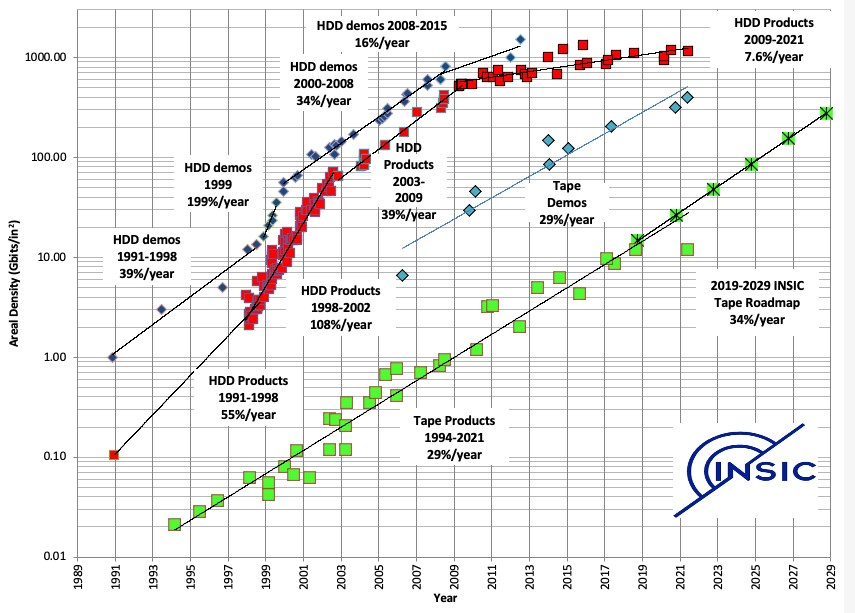
\includegraphics[width=\linewidth]{Figures/INSIC-2022-Areal-Density-Chart.jpeg}
    \caption{Density trend of HDD and Tape during years and the estimation of this trend till 2029}
    \centering
    \label{fig1}
\end{figure}
\subsection{Storage maintenance and replacement}
To link to the previous paragraph, HHD device has short lifespan: almost from 3 up to 5 years before the need to replace it. Data stored in any modern storage devices are periodically re-written onto new generations of devices as well in order to ensure continued access and to provide a better user experience.
Notwithstanding, not all kind of data needs this continuous accessing (better explanation in the two next paragraphs), hence rewriting periodically this data and updating the storage device have higher costs during the time. Consequently a lot of companies are pushing experts to create new kind of long-term storage devices.

\subsection{Energy consumption of digital storage device}    Some studies done in the USA in 2006 indicates that data centers consumed almost 1.5\% of the total energy, this is estimated to be the consumption of 5.8 million average people in the United States for an amount of 4.5 billion dollars.Additionally, the power required by the country's servers and data centers in 2006 was more than twice as much as it was in 2000 \cite{shehabi2016united}. Additional research comparing several projections reveals the potential trajectory of energy usage.

In the “best-case scenario” the energy consumption of data centers can remain constant during the time or at least increase slightly. Anyway, since Moore's general Law, as said before, cannot be applied and the performance of the data centers increases significantly, there could be an increase in energy consumption of up to 3,000 billion kWh/year. As a consequence, the consumption of data centers will double by 2030 compared to today \cite{hintemann2019energy}.
It is possible to see this trend in the Figure \ref{fig2})

\begin{figure}[ht]
    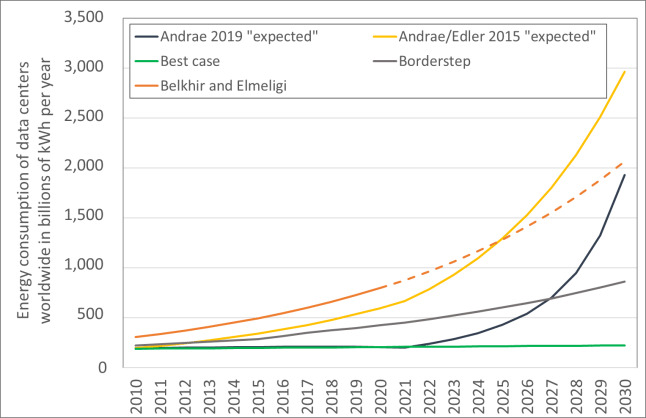
\includegraphics[width=\linewidth]{Figures/Energy-consumption-of-servers-and-data-centers-worldwide-forecasts-to-2030-A-comparison.jpg}
    \centering
    \caption{Energy consumption of data centers over year and its estimation till 2030 \cite{inproceedings}}
    \label{fig2}
\end{figure}

\subsection{Hot-data vs Cold-data}
Storage can be divided into 2 huge different categories: hot data and cold data.
Hot data are data accessed frequently. They are stored in high-performance devices, such as RAM, SSD, and cache, that need frequent access in order to write and read on the memory and need a high temperature to work in the best possible way. A well-known example may be computers whose components exceed 20 Celsius degrees in temperature up to 80.

On the other side, cold data are data accessed less frequently, consequently, they need less heat. Most of the time they are stored on tape + HDD, which may be seen as a huge waste of space and energy consumption.

Such division is fundamental since in recent years a trend is represented by the fast growth of the amount of cold data compared with hot data, mostly, this is due to the fact that people need to store more data for a longer period of time. Moreover, it is common that less than 1\% of this data is accessed more than 90-120 days after its creation\cite{alliance2021preserving}. 

In between, we might refer some data as warm data which are neither hot nor cold. In other words they are a kind of data which are not going to be used by user often and are not the data that might not be used for ever.

\section{DNA: An alternative data storage medium}
\label{sec:DNA: An alternative data storage medium}
Considering the massive accumulation of digital data plus the physical requirements and amount of carbon used by other storage methods, researchers felt the need for another storage alternative. Little by little minds were diverted towards DNA storage \cite{choi2019high}. The first person who experimentally tried to construct DNA storage was Joe Davis who converted a 35-bit image of the ancient Germanic rune for a female goddess "Microvenus" to a $5\times7$ matrix of 0's and 1's. The 0's show the brighter parts, while the 1's show the darker parts and encoding this binary data into 28 base pair (bp) DNA molecules. After his research, other methods were proposed in various papers including converting binary data to nucleotides A, C, G, and T synthesizing the sequence, and storing the data afterwards \cite{dong2020dna}.

One of main advantages of using DNA as a digital data storage are:
\begin{itemize}
    \item DNA has the potential of storing petabytes of data per gram which means a very high information density.
    \item Data can be stored for a long-term (centuries) without degradation which is obviously suitable for cold data.  
\end{itemize}

The above reasons made the researchers determined to continue working on this method, hence different approaches of DNA storing techniques \cite{grass2015robust}.

\section{DATA TO DNA: THE DIGITAL DATA PIPELINE }
\label{sec: DATA TO DNA: THE DIGITAL DATA PIPELINE}
DNA storage has its complexity but by dividing it into different stages we can understand and focus better the procedure.

Storing data into DNA molecules consists of the following steps:
\begin{itemize}
    \item Binarization: Different type of data can be stored like videos, photos, musics, web-pages, and etc. In the first step they should be changed to binary strings or matrices.
    \item Encoding: Encoding is the process of converting binary data into DNA nucleotides.
    \item Synthesis: The way of placing the encoded data to DNA strands is known as synthesis. In other words, writing the data into DNA.
\end{itemize}

On the other hand, the process of retrieving data from DNA needs the steps below:
\begin{itemize}
    \item Sequencing: DNA sequence analysis involves determining the identity and order of DNA bases (ACGT).
    \item Decoding: It's exactly the opposite of the encoding stage which the nucleobase codes are converted to binary code.
    \item Reading: After decoding process is finished, the data is put back together and sent to the user as a digital file.
\end{itemize}

Due to the existence of successive stages we introduce the whole process as a pipeline which are briefly visualized in the figure \ref{fig3}. 
\begin{figure*}[ht]
    \centering
    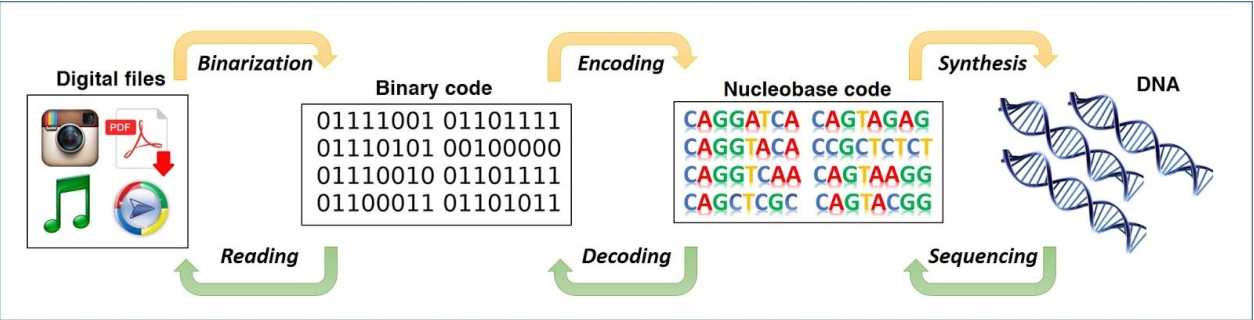
\includegraphics[width=\textwidth]{Figures/pipeline.png}
    \caption{The process of storing and retrieving data through DNA molecules \cite{Swati2017ARO}}
    \label{fig3}
\end{figure*}

Here we will focus on encoding and decoding more than the other parts because working with DNA does not only need engineering knowledge but also biology expertise as well. However, it doesn't mean that these two section are independent from other sections because the methods used for synthesis and sequencing might affect our efficiency. In the next subsection it will be discussed more.

\section{Encoding}
\label{sec: Encoding}
We are encoding data using a code in order to modify it into a form that can be used in an external project, in our case to store data in DNA molecules.

Anyway, to have a general overview of this process, it is important to introduce the most general case code used for converting characters, which is also known as ASCII (American Standard Code for Information Interchange), the most commonly used encoding scheme for files, where a unique number is assigned to some characters. ASCII contains 2 different types of characters: This includes symbols, punctuation marks, numbers, and upper and lowercase letters that can be printed and those that cannot.
The audio and video files are additionally resized using encoding.

Furthermore, encryption, which conceals content, should not be mistaken with encoding. Both methods are widely employed in the sectors of networking, software development, wireless communication, and storage. Different encoders may then use different rules to convert bits to sequences. The rule of thumb for conversion is to avoid repeating bases (homopolymers) and to include primer target sites at both ends \cite{technopedia2021}.

\subsection{Error Correction Codes}
While doing the encoding process we need to remark that errors might happen, hence an error correction code is needed which increases the probability of the original information to be retrieved even in the presence of errors or missing data. The process typically involves computing a summary of the data and storing and/or transmitting it with other data and using the redundant information to correct errors generated. An inner code refers to coding within a single strand to correct local errors. An outer code instead refers to whole new additional strands that deal with errors and which are not covered by inner codes, an example may be erasures\footnote{The removal of writing recorded material or data.}.

The basic idea of error correction is to embed redundancy to the original data (Figure \ref{fig4}). The resultant storage method will be more error (or loss) tolerant the more redundancy there is. There are two main categories of redundancy that apply to this:
\begin{itemize}
    \item Physical redundancy: that is to have copies of the DNA sequence many times so that in the time of retrieval losing data will decrease.
    \item Logical redundancy: is the results of mathematical manipulation of data to correct errors inserted in the data as bits are stored, transmitted, and so on when encoding data in the DNA sequences. A logical 'exclusive-or' operation is needed and maybe sometimes a pseudo-random number generator that ensures DNA strands are dissimilar.
\end{itemize}

Some of the error correction methods which is done in our case study papers can be seen in the Table \ref{tab:error correction}.

\begin{figure}[ht]
    \centering
    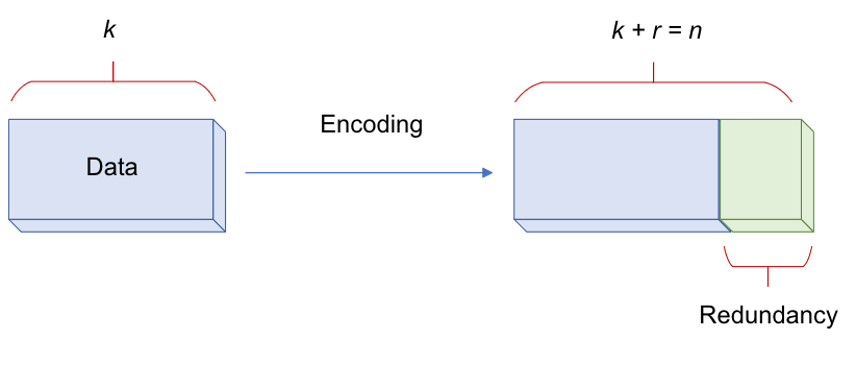
\includegraphics[width=\linewidth]{Figures/encoding.png}
    \caption{Encoding using error correction. Consider Data with the length k. A redundancy with the length r will be added for the process of error correcting so, the overall embedded code will be with the length $n=k+r$}
    \label{fig4}
\end{figure}

In a nutshell, reliable data storage and retrieval need error correction methods for all types of media (and communication channels such as radios). In this case, it is possible to mention a whole field of computer science called information theory, or coding theory, that focuses on developing coding schemes able to deliver digital data reliably over noisy media and communication channels.

These sequences may go through a logical ‘exclusive-or’ operation with a pseudo-random number generated from a known seed to ensure that DNA strands are dissimilar, and then redundancy is added via codes, such as Reed–Solomon codes, for error correction purposes.

\subsection{Error-Prone Steps}
DNA storage is different from other techniques for the following reasons:
\begin{itemize}
    \item Having substitution errors
    \item Manifesting base insertions and deletions
\end{itemize}

Moreover, DNA synthesis and sequencing are error-prone. The error rate per base per position reported in several papers analyzing DNA data storage is approximately 1\%. More precisely, for a given position in a DNA strand, when synthesized and sequenced back, approximately 1\% of the reads will have an error in that position.
\section{Error Correction Methods}
\label{sec: Error Correction Methods}
The first error-correcting methods goes back to 1940s. Receivers, which are stated a level before the user can use this extra redundant data to check whether the received message is consistent and, if it is not, to potentially reconstruct the original data. The amount of redundant data to be added can vary depending on the noise profile of a channel, on the code used, and on the desired probability of successful decoding.

Overall, the error correction methods can reach to the following criteria which also can be seen in Figure \ref{fig5}:
\begin{itemize}
    \item The encoding method should handle the bad events and prevent corruption during the encoding process.
    \item should have the ability to recover the original data through adding the redundancy
    \item Although adding the redundancy increase the fault tolerant, it increases the overhead which is costly. So, the selected method should minimize the overhead (Overhead: $k/n$).
    \item at last, the process of encoding should be efficient regarding the physical footprint and the time consumption.
\end{itemize}

\begin{figure}[ht]
    \centering
    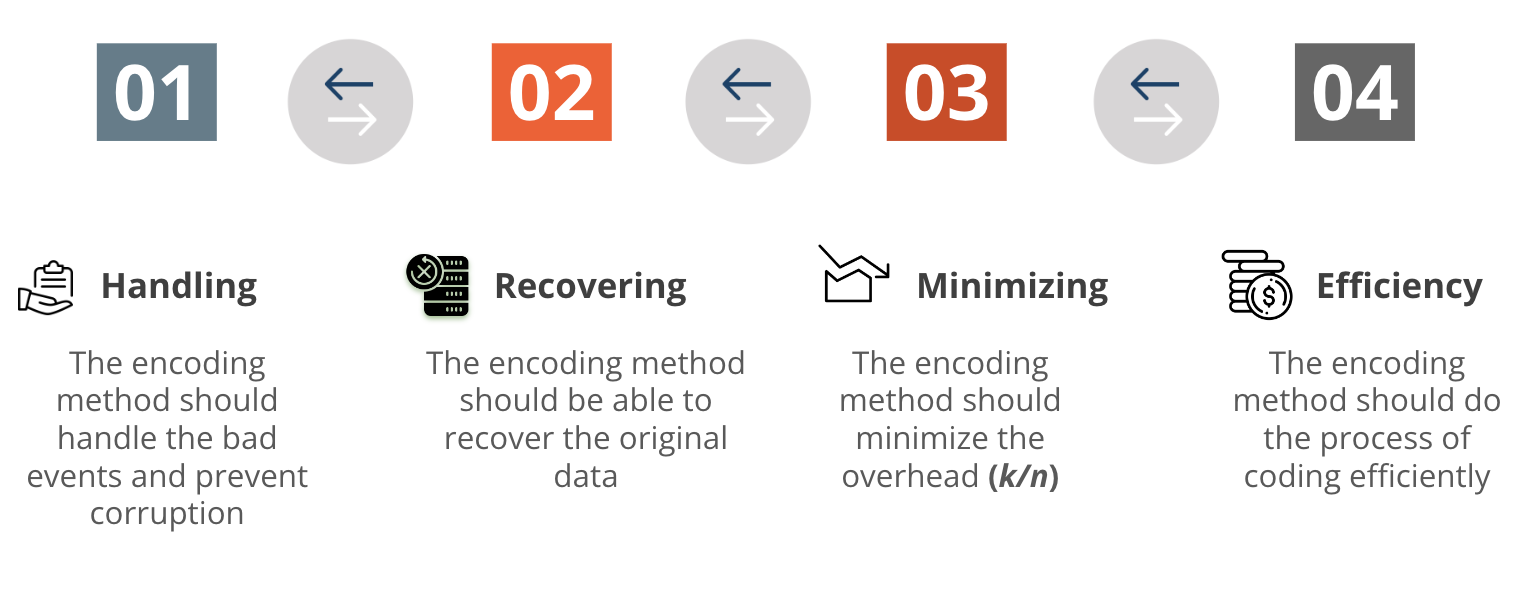
\includegraphics[width=\linewidth]{Figures/Encoding goals.png}
    \caption{Trade of between different aspects might be considered while using the error correction in the process of encoding}
    \label{fig5}
\end{figure}
In the next subsection one of the most powerful methods according to the goals of the error correction will be explained. It is good to note that all of the error correction methods have the background of algebra in themselves. So we will refuse to explain all the definitions regard that.
\begin{table*}
\centering
\caption{Methods of Error Correction}
\begin{tableminipage}{\textwidth}
\begin{tabularx}{\textwidth}{@{}XXX@{}}
\hline
{\bf Type} & {\bf Description} & {\bf Goal}\\
\hline
Physical Redundancy & Joined overlapping paired-end 100-nt reads & Retrieve data correctly\\
Logical Redundancy & Reed - Solomon (sequences may go through a logical ‘exclusive-or’ operation For DNA strands to be dissimilar, a pseudo-random number is generated from a known seed, and then redundancy is added via codes)
 & Handle erasures and errors\\
Logical Redundancy & Shifting Pattern (a piece of data is repeated at different offsets in different DNA sequences) & avoid systematic errors
\\
Logical Redundancy & Multiple pieces of information are summarized into one or more additional pieces by a XOR operation & Handle Overhead
\\
\hline
\end{tabularx}
\label{tab:error correction}
\end{tableminipage}
\end{table*}
\subsection{Reed-Solomon}
Reed-Solomon codes are a family of $(n,k,q)_{d}$ that:
\begin{itemize}
    \item achieve the singleton bound $(n=d+k-1)$
    \item admits efficient encoding and decoding algorithms
    \item are used all over the place in practice
\end{itemize}

The idea behind reed-solomon codes is low degree polynomials that don't have too many roots. It is especially important that the code words of read solomon code consist of evaluations of low-degree polynomials so that there are not too many zeros in them resulting in good code distance. To be more precise we have the definition of reed-solomon codes as follows:
\begin{definition}[Reed-Solomon Codes]
\ Let $q\geqslant n\geqslant k$.
\\ Let 	$\alpha_{1},...,\alpha_{n}\in F_{q}$ , with evaluation points $\overrightarrow{\alpha}=(\alpha_{1},...,\alpha_{n})$, is:
\begin{center}
$RS_{q}(\overrightarrow{\alpha},n,k)=\{(f(\alpha_{1}),f(\alpha_{2}),...,f(\alpha_{n})):f\in F_{q}[X], deg(f)\leqslant k-1\}$
\end{center}
\end{definition}
So the read-solomon code of dimension k with evaluation points alpha is the set of all such vectors.
Reed-Solomon has the following properties:
\begin{itemize}
    \item They are linear codes with Vandermonde matrices as generator matrices which has n rows and k columns.
    \item The distance of $RS_{q}(\overrightarrow{\alpha},n,k)$ is exactly $d=n-k+1$.
    \item One of the most important characteristics of reed-solomon codes is exactly meeting the singleton bound, which we refer to as maximum distance separable (MDS).
\end{itemize}

In \cite{grass2015robust} DNA can be used as a storage medium for digital information and be recovered without error over a much longer period of time. Error-correcting codes are encased in an inorganic matrix to correct mistakes associated with memory. The nucleotides were encapsulated in silica. It was possible to restore the original information after treating the DNA in silica at $708^\circ C$ for a week without errors.

This case study's main concept was as follows: As shown in Figure \ref{fig6}, individual sequences are indexed, and two independent error-correcting codes (particularly Reed-Solomon codes) are employed in a concatenated manner.

\begin{figure*}[ht]
    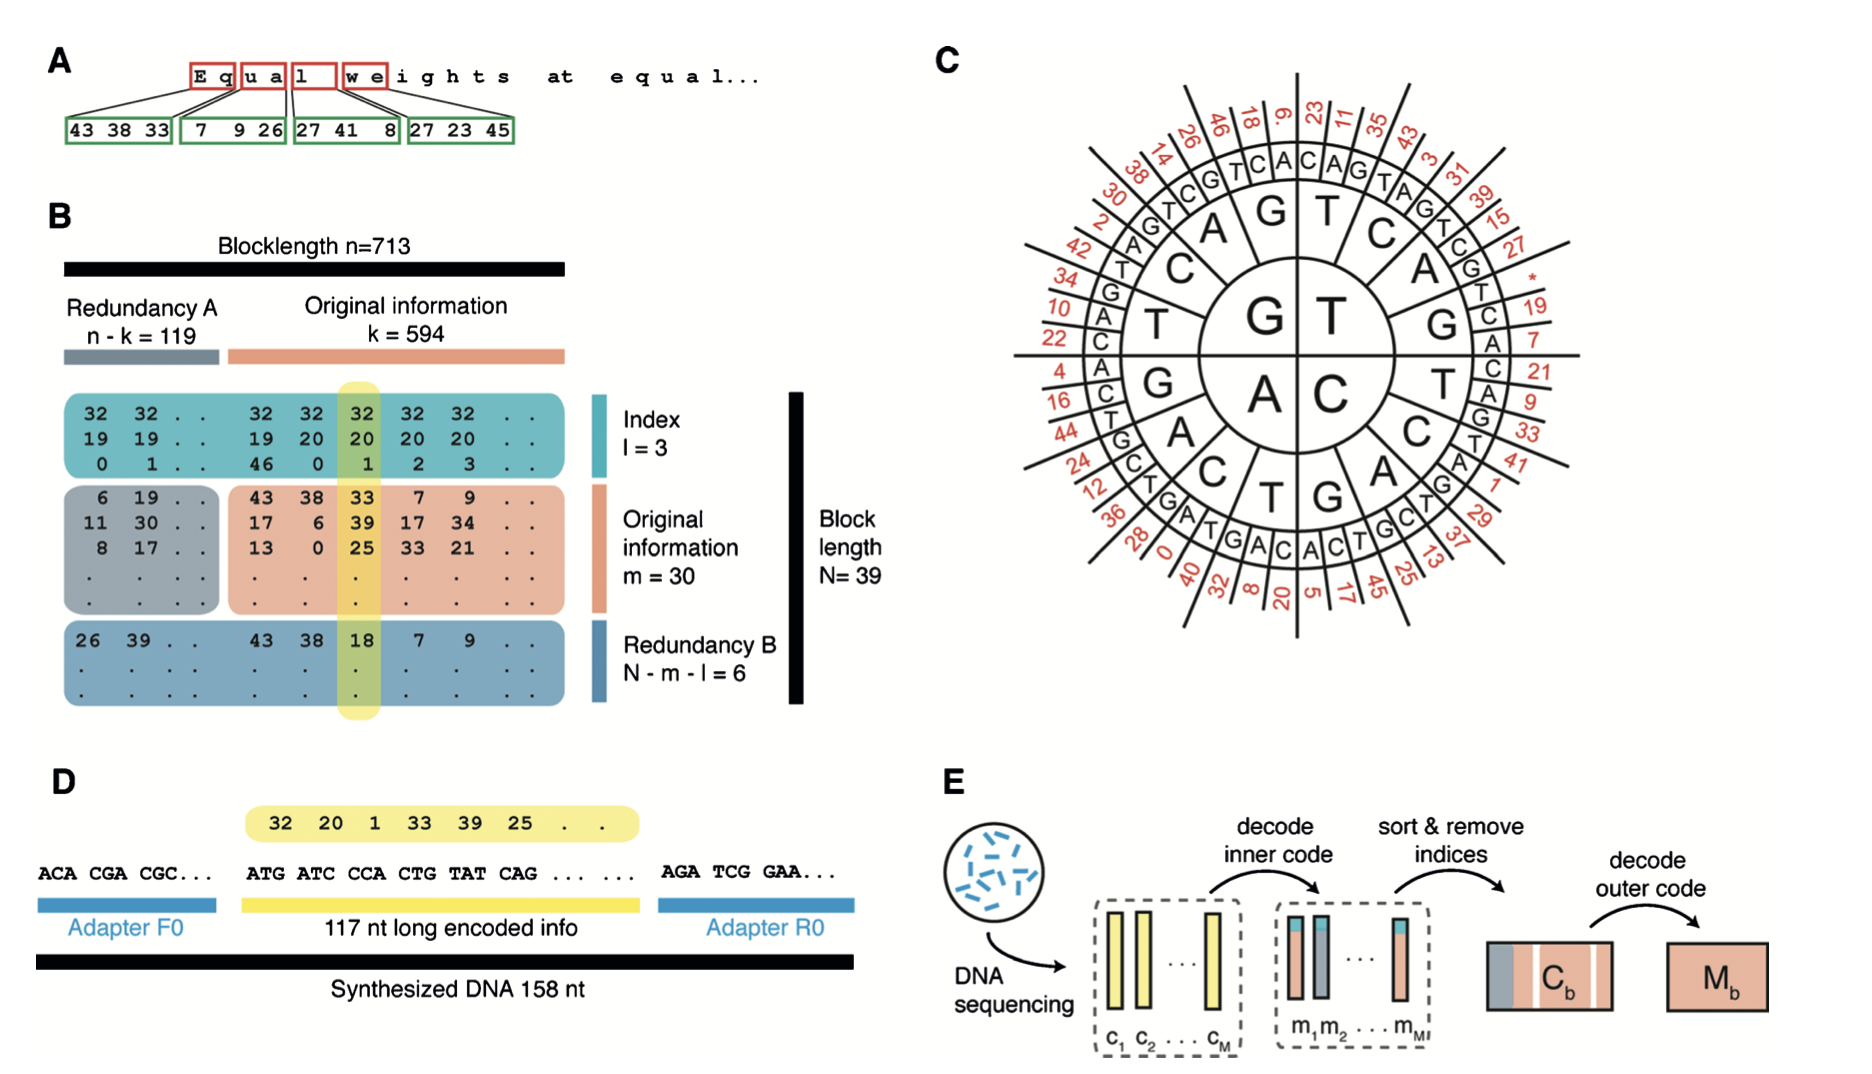
\includegraphics[width=\linewidth]{Figures/reed-solomon-error-correction.png}
    \caption{Encoding text to DNA by Reed–Solomon coding: A) Using base conversion (2562 to 473), two letters in a text file (or more generally, two bytes in a digital file) are mapped to three elements in the Galois Field of size 47 (GF(47)). A block of \(594 \times 39\) elements is used to organize this original information. B) To add redundancy A to each block, Reed-Solomon (RS) codes are employed in an outer encoding step. Redundancy B is generated by adding an index to each column and using a second (inner) RS encoding step. C) With the help of the GF(47) to DNA codon wheel, every column is converted into DNA by mapping each element to three nucleotides, ensuring that no base is repeated more than three times. D) The resulting sequences of 158 nucleotides are synthesized by adding two constant adapters. E) For the recovery of the original information from the DNA, the read sequences are translated to GF(47) and decoded by first decoding the inner code (correcting individual errors), sorting the sequences by index, followed by outer-decoding, which allows the correction of whole sequences and the recovery of completely lost sequences (see the Supporting Information for details on coding and experimental procedures).}
    \centering
   \label{fig6}
\end{figure*}

\section{Shannon Information As a Metrics}
\label{sec: Shannon Information As a Metrics}
DNA storage is a communication channel that receives data by sequencing the oligos\footnote{Oligonucleotide}. In any case, the channels are noisy as a result of a number of DNA encoding steps, including imperfect DNA synthesis, PCR dropout, stutter noise, sequencing errors, and even the gradual degradation of DNA molecules over time, also known as experimental factors.

When compared to their binary counterpart, where the noise is identical and randomly distributed, these errors are significantly different; instead, the DNA error pattern greatly depends on the input sequences.
Anyway, a lot of previous studies on the error pattern show that the running homopolymer and the GC content are the major determinants of synthesis and sequencing error.

Shannon provides results about resources needed for optimal coding and error-free communication and helps to measure the quality of DNA storage encoding.

Here there is an explanation of how it works.
According to Shannon exist a general communication system:
\begin{itemize}
    \item A Source $S$, which generates the message.
    \item A Transmitted $T$, which turns the generated massage into a signal to be transmitted.
    \item A Channel $CH$, that is, the medium used to transmit the signal from the transmitter to the receiver.
    \item A receiver $R$, which reconstructs the message from the signal.
    \item A destination $D$, which receives the message.
\end{itemize}

In the sorce $S$ there is a range of possible state starters $s_{1},..., s_{n}$ called $Latters$, and their respective prob are given by $p(s_{1}),...,p(s_{n})$ .
So the amount of information generated is defined as:
\begin{center}
$I(s_{i}) = \log(1/p(s_{i})) = - \log(p(s_{i}))$
\end{center}
Since $S$ produces sequences of state called messages, so the full entropy of the source S is defined as using the minus form:
\begin{center}
$ H(S) = - \sum_{i = 1}^{n} \log(p(s_{i}))$
\end{center}
Analogously we have the same value for the destination $D$ so y $d_{1},..., d_{m}$ the range of destination reached, with the respectively probabilities $p(d_{1}),...,p(s_{m})$. At the destination, the quantity of information is calculated as:
\begin{center}
$I(d_{j}) = \log(1/p(d_{j})) = - \log(p(s_{j}))$
\end{center}
and its $entropy$ it s defined:
\begin{center}
$ H(D) = - \sum_{j = 1}^{m} C$
\end{center}

Furthermore, looking at the previous formulas, it is possible to notice that a logarithmic function is used, because mathematically the log function is more suitable due to many limiting operations in log which are easier. Moreover, by choosing a base 2, the resulting amount of information obtained is called $bit$ that is the UNIT in digital storage.
In-depth on the specifics, below is the amount of knowledge discovered about two equally likely specified options.
The image above shows the relation between the source information $H(S)$ and the destination $H(D)$:
\begin{itemize}
    \item $H(S;D)=H(S) \cap H(D)$ is the $mutual information$ the amount of information generated by the source and correctly received by the destination
    \item $E=H(S) \backslash H(S;D)$ is the $equivocation$ the amount of information generated by source but not received by destination.
    \item $N=H(D) \backslash H(S;D)$is the $noise$ the information received by the destination but not generated by the source.
\end{itemize}

In addition, Shannon's information does not depend only on the information sent and received but it is also necessary to take into account the $CH$ crossed transmission channel. In the case analyzed in this paper, the channel is the synthesized DNA molecule. The risk of transmission mistakes is instantly introduced with the creation of the communication channel..

As a conclusion, it is possible to take into account those errors by defining the matrix $[p(d_{j}\backslash s_{i})]$ where $p(d_{j}\backslash s_{i})$ is the conditional probability of the $d_{j}$ in the destination. As a consequence, it is possible to compute N and E in the following way:
\begin{center}
$ N = \sum_{j = 1}^{m} p(s_{i}) \sum_{i = 1}^{n} (p(d_{j}/s_{i})) \log(1/p(d_{j}/s_{i}))$
\end{center}
\begin{center}
$ E = \sum_{j = 1}^{m} p(d_{j}) \sum_{i = 1}^{n} (p(s_{i}/d_{j})) \log(1/p(s_{i}/d_{j}))$
\end{center}
where $p(s_{i}/d_{j}) = \frac{p(d_{j}/s_{i})p(s_{i})}{p(d_{j})}$.

The $CH$ $capacity$ is defined as: 
\begin{center}
    $C = max_{p(s_{i})}{H(S;D)}$
\end{center}

The maximum is taken all over the distribution $p(s_{i})$ from the source, instead, $C$ measures the larger amount of information that can pass over the communication channel $CH$.

For summaries Shannon provides two important theorems to measure information transmission:
\begin{itemize}
    \item $First Theorem$ or $Noiseless-Channel Coding$, in order to have a sufficiently long message, the value of $entropy (H(S))$ should be equal to the average number of symbols necessary to encode one letter of the source (GTAC) by using an ideal code.
    \item $Second Theorem$ or $Noisy-Channel Coding$ says that the channel capacity is equal to the maximum rate at which the information is sent and retrieved at the destination with a very low probability of error.
\end{itemize}
Further details on Shannon can be found \cite{lombardi2016shannon}.

\subsection{Definition Of Information Capacity}
It is feasible to provide a simpler explanation of the term "Bytes per bases" by skipping over some of the arithmetic that underlies Shannon and the definition of the information capacity: "The input information in bits divided by the number of synthesized DNA nucleotides."

Even though the unit for the term is slightly different in the literature, the parameter is used to determine how much data can be encoded in the DNA sequence, before the synthesis of the DNA itself. Therefore, it is a value that can intuitively convey the performance of data to the DNA by encoding algorithm.

\begin{center}
    $\frac{\log_{2}(K)}{l} bits/character $
\end{center}
$K$ $=$ $Numbers$ $of$ $codon$

$l$ $=$ $Numbers$ $of$ $base$ $per$ $codon$

Example of usage:

To use 15 basis $"A,T,G,C,Y......"$ so 750 codons are generated $(K)$ $ATC,ATY,ATG ....$ in 3-base-codons $(l)$ are generated.

From this term should be multiplied other factor terms that depend on the encoding strategies and the error correction coding used.

In the following figure (Figure \ref{fig7})  the real information density in comparison to best mapping potential is shown.
\begin{figure}[ht]
    \centering
    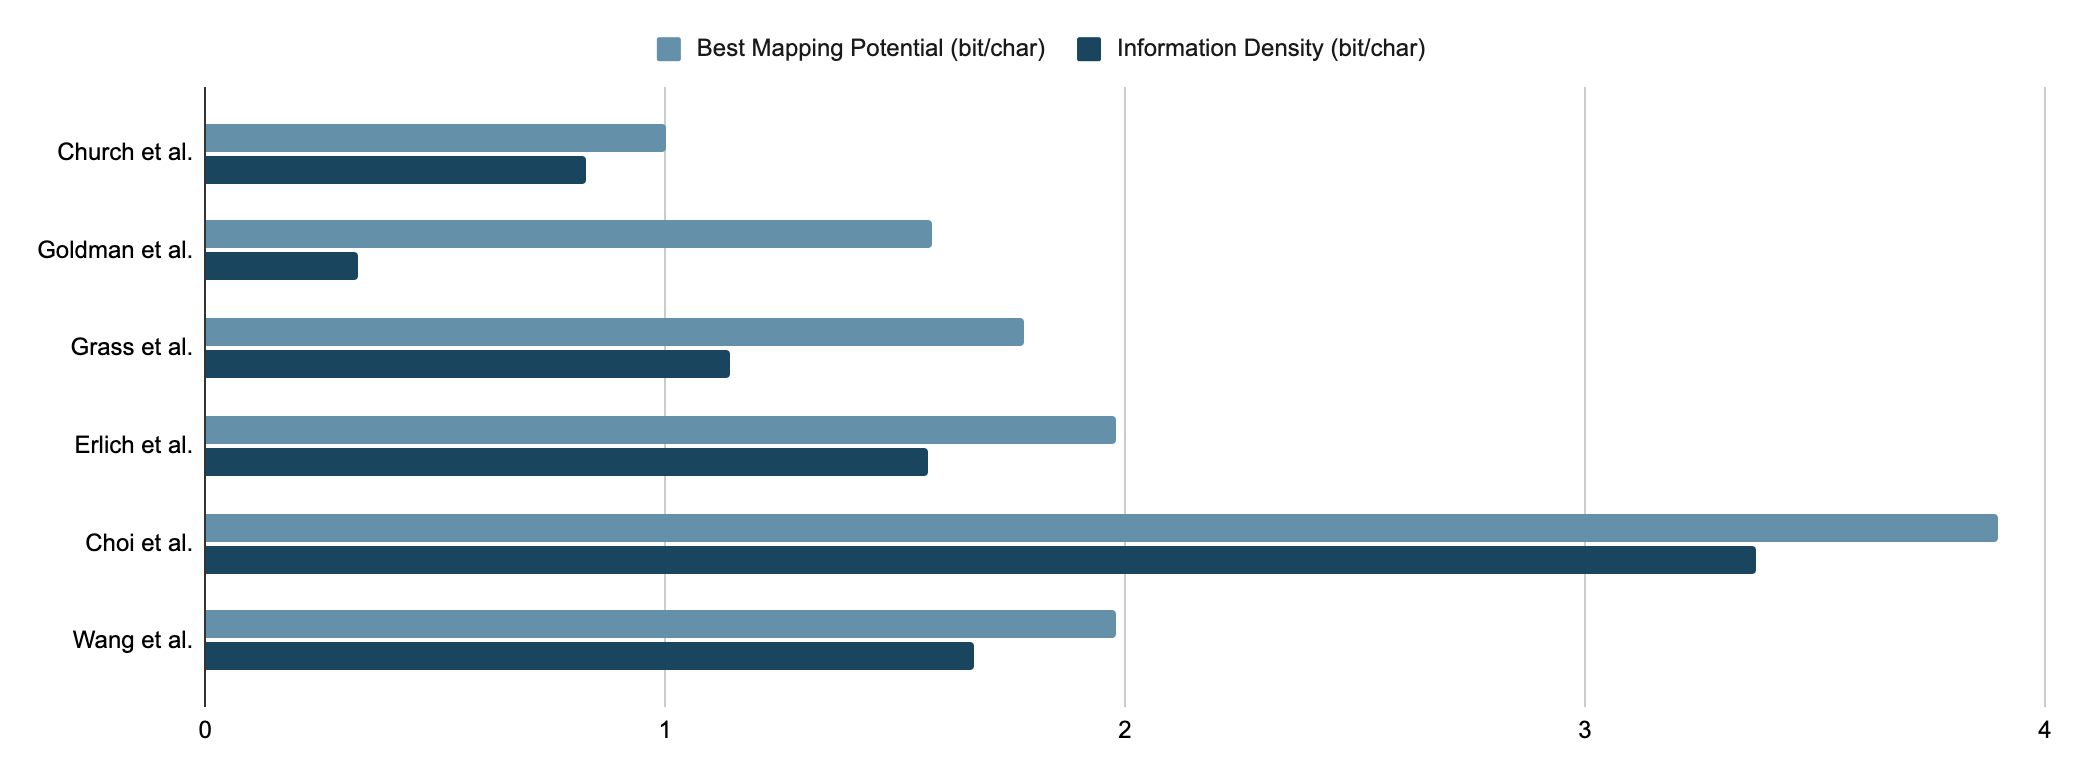
\includegraphics[width=\linewidth]{Figures/information.png}
    \caption{Analogy between the information capacity in some of the case studies and the theoretical boundary calculated from Shannon information.}
    \label{fig7}
\end{figure}


\section{Encoding Approaches}
\label{sec: Encoding Approaches}
In the following sections some of the recent and important approaches which have the proper results considering the theoretical Shannon information are going to be explained. The selected approaches are based on the comparison showed in figure \ref{fig7}.

\section{DNA Fountain approach}
A study conducted by Y.Erlich and D.Zenlinki in 2017 has changed the way of coding the information into DNA molecules and in some cases, it was possible to retrieve perfectly the information.

The technique they used is known as DNA Fountain. 
The tactic uses fountains codes, which enable accurate and efficient information unicasting over dropout-prone channels, that are subject to dropouts. It is possible to divide the technique into 3 parts:
\begin{itemize}
    \item A binary file is processed in the first step into a series of segments that are $non-overlapping$ and $segment$ of a fixed length. The segments are then packed into a single tape-archive file, which is then compressed using a standard lossless algorithm.
    
    \item At this point the $Luby$ $Transform$ $Algorithm$ is applied, it sets the basis and prepares them for the fountain transform. Additionally, it organizes the data into units called droplets, chooses them using a unique distribution, and then adds them bitwise under a binary file.
    The droplets contains two pieces of information:
    
    \begin{itemize}
        \item $data$ $payloads$ that holds the result of the addition procedure.
        
        \item $fixed$ $length$ $seed$, this seed is randomly generated from the distribution mentioned above and this allows the decoder algorithm to infer the identities of segment droplets.
    \end{itemize}
    
    \item The program then advances to the $screening$ phase, when it transforms the binary droplets from ${00, 01, 10, 11}$ to ${A, G, G, T,}$ translating them into a DNA sequence. Then it screens the sequence, and whether it passes the screening it is considered valid and added to oligos design files, otherwise, it gets discarded.
    It is possible to iterate this step until it is not found a correct amount of valid oligos. 
\end{itemize}
Most importantly, Erlich and Zenlinki have been able to achieve an information density of $1.57bit/nt$ which was a huge improvement from the previous studies that instead achieved a density of a maximum $1.14bit/nt$.

\subsection{Luby Transform Algorithm}
\begin{enumerate}

    \item First initialize a $pseudorandom$ number generator $PRNG$ with a seed. The seed is selected by a mathematical rule.
    \item The algorithm decides on $d$, the number of segments to package into the droplet. To do this the algorithm calls the PRNG function that draws a random number from a special distribution function (more details in the paper).

    \item The algorithm uses again the PRNG to draw d segments but in this case with a uniform distribution and without the replacement of the previous draw.

    \item The algorithm performs a bitwise-XOR operation mod 2 on the segments.
        \begin{center}
            \[ XOR(x,y) =
                \begin{cases}
                    0 & \text{if } x = y\\
                    1 & \text{if } x \ne y
                \end{cases}
            \]
        \end{center}
    where x and y the bits is the same position but from the different string of bits, example( $0010$ XOR $1010$ = $1000$).

    \item The technique also generates a fixed-length index that describes the seed's binary form. For instance, the output droplet will be $10$ $+$ $1000$ if the seed is 1 and the fixed index length is 2 bits, where 10 is the binary $2^{0}$ encoding of 1.

    \item The user can choose between using a standard error-correcting code calculated on the entire droplet or the popular Reed-Solomon error-correcting code \cite{erlich2017dna}.
\end{enumerate}

\section{Degenerate Basis Approach}
DNA with a degenerate basis is trying to solve a big problem of the maximal information stored inside a sequence of DNA, For example, previous studies try to fix this problem by developing a cheaper synthesis phase, because of the cost of writing (storing the data) is really huge, or at least try to find a better encoding algorithm. However, maximizing the amount of data that may be stored per length of the intended DNA sequence is the simplest and most easy approach. More detail in Figure \ref{fig8}. 

By looking at the DNA Fountain approach done by Erlich and Dina Zenlinki they were able to have a theoretical information capacity limit of $\log_{2}(4)$ or $2bits/character$.

By the way, if in addition to the standard encoding oligos introduced the degenerate basis, the information capacity of $\log_{2}(number of encoding characters)$ drastically increases, so it reduces the cost of the DNA data storage.

Degenerate bases are stored in the DNA sequence when oligos are grouped together at some specific position in the sequence of the DNA. For example:

$"AWC"$ where $"A"$ and $"C"$ represent their specific oligos and W represent as said before a mixed pool of $"A"$ and $"T"$. Moreover, it is possible to define 2 types of nucleotides $"AAC"$ and $"ATC$ 

So by using these methods it is possible to achieve a better result in terms of information capacity of $3.37 bits/nt$.
The Figure \ref{fig9} it is presented the structure of the DNA-based data storage used for DNA coding \cite{choi2019high}.

\begin{figure*}[ht]
\centering
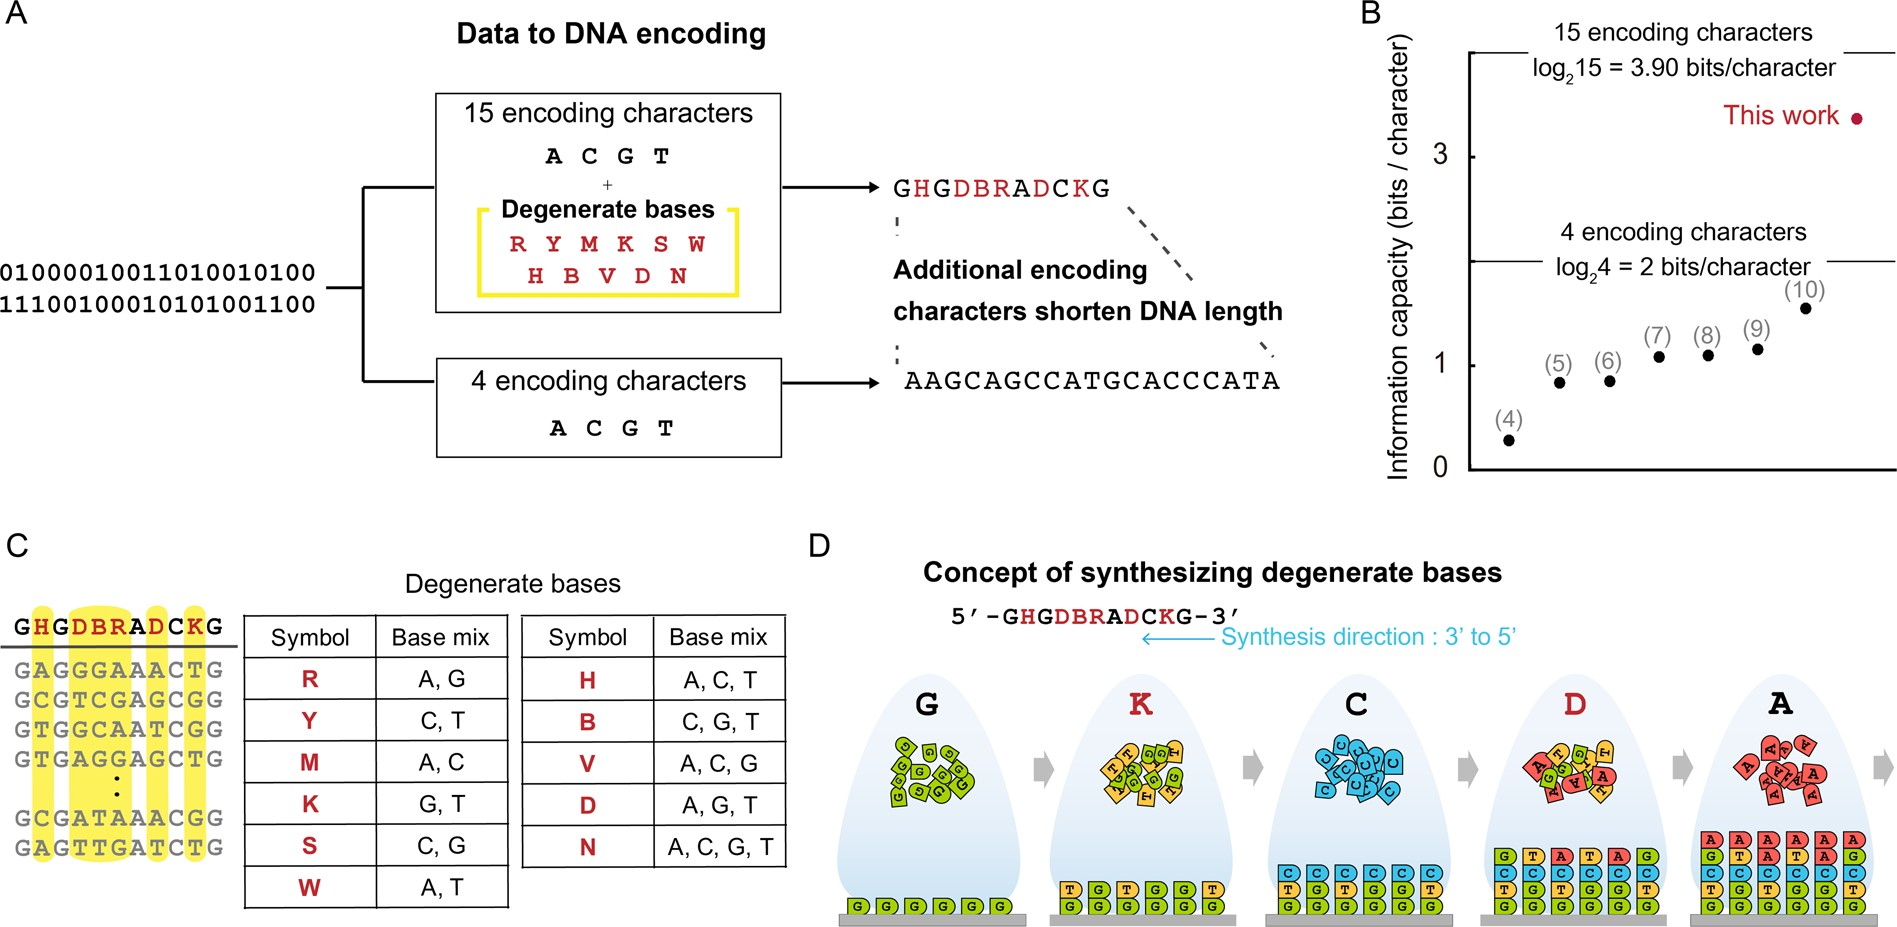
\includegraphics[width=\linewidth]{image degenerate basis.jpg}
\caption{The addition of degenerate bases increased information capacity the image explanation is given by \cite{choi2019high}.
\\(A) Binary data is encoded to DNA sequences comprising not only the 4 traditional encoding characters A, C, G, and T but also 11 additional degenerate bases. But instead, the length of the encoded DNA is shorter than the four-character encoding method.
\\(B) Furthermore the theoretical information capacity is increased from 2 bits/character to 3.9 bits/character. The dots describe the information capacity values in previous research, more precisely the last one refers to the DNA fountain approach that scores the best value.
\\(C) A degenerate base represented by an encoding character describes a mixed pool of more than two types of nucleotides, so it is possible to store more information in each oligo.
\\(D) Degenerate bases can be generated by mixing the DNA phosphoramidites during the synthesis procedure.}
\label{fig8}
\end{figure*}

\begin{figure*}[ht]
\centering
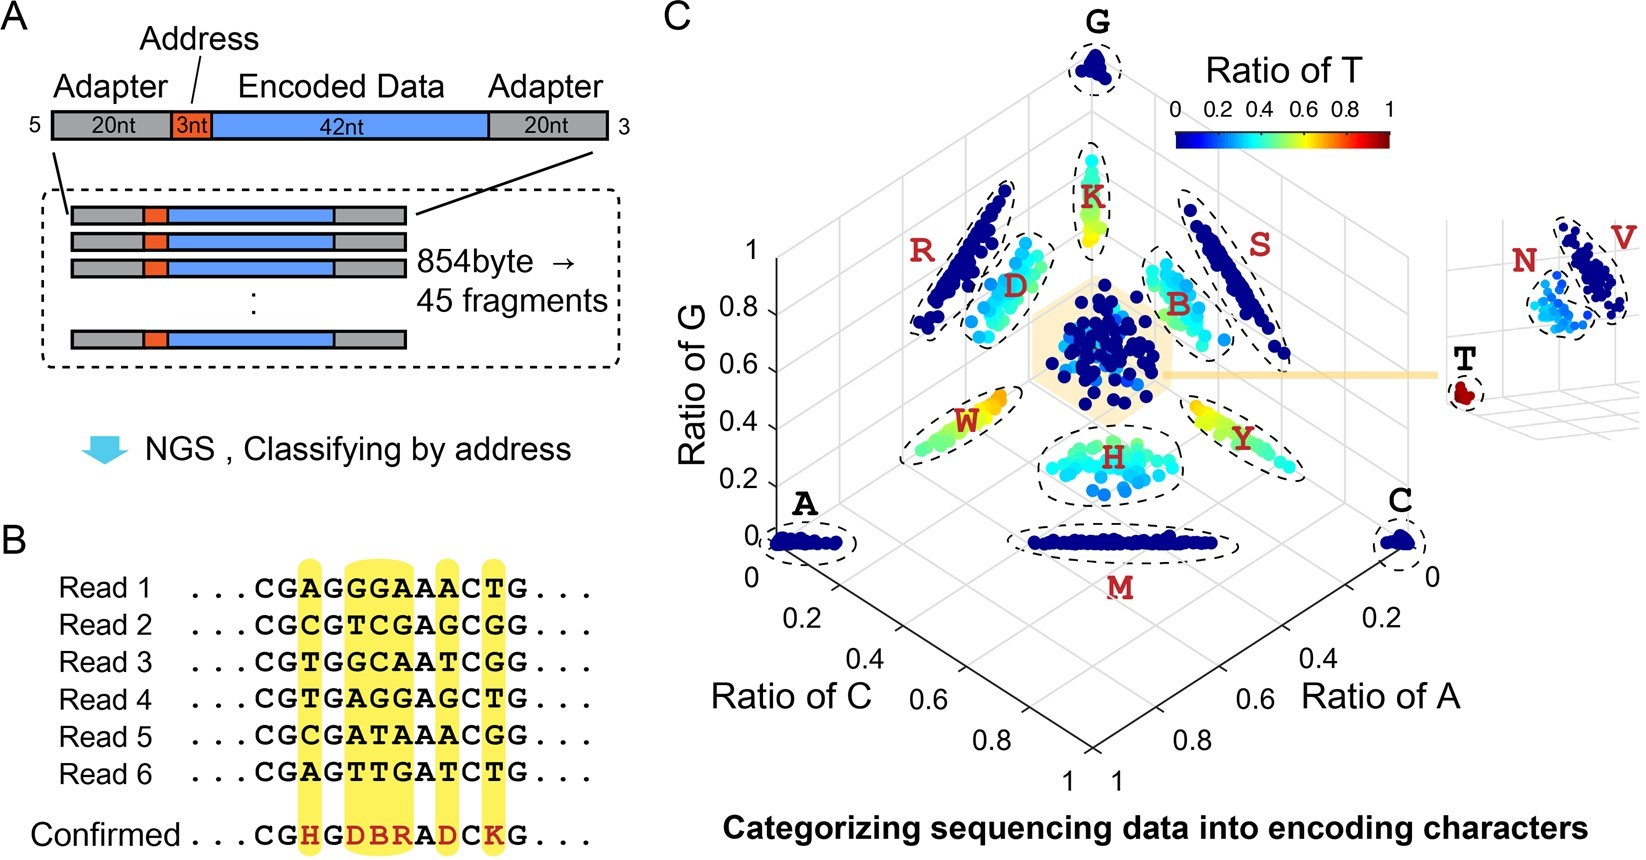
\includegraphics[width=\linewidth]{other on degenerate basis.jpg}
\caption{ The above illustration tries to give a better explanation of degenerate basis encoding taken from the \cite{choi2019high} that explain all the process behind.
\\(A) Design structure of DNA fragments. \\(B) DNA fragments can be analyzed using NGS. After classification by address, degenerate bases can be decoded by examining the distribution of characters in the same position (yellow bar). \\(C) Degenerate bases can be determined from the scatter plot of the ratio of bases in the same position}
\label{fig9}
\end{figure*}

\section {Variable length oligonucleotides Approach}
The older paper explored finds a lot of problems, in particular, they dealt with two big issues that have to be faced in DNA data storage. 

The first step is to create the right error correction coding to address the faults brought on by the pipelines for synthesis, storage, sample preparation, and sequencing.

The second deals with designing a DNA mapping approach that, subject to specific biological restrictions, converts binary files into DNA sequences.

Moreover, by looking at the 2 precedent approach proposed by The DNA Fountain and the addition of the degenerate basis, it is true that really high $bits/nt$ is reached but necessitates higher sequencing improvement and also synthesis techniques for practical usage.

Additionally, this approach does not start from the degenerate basis but it starts from the DNA fountain and tries to improve the solution given by Yaniv Erlich and Dina Zenlinki.

To overcome the limitation of DNA fountain, this approach explores another practical common error and really efficient DNA mapping strategy. In particular, the hybrid mapping scheme consists of 2 different mapping methods: 
\begin{itemize}
    \item Interval mapping.
    \item variable-length constraint $VLC$ mapping.
\end{itemize}
they are create to reach the optimal $2bits/nt$ while balance 2 important constraint:
\begin{itemize}
    \item $"GC"$ content.
    \item and $maximum homopolymer run$ limit.
\end{itemize}
Furthermore, a packet-level called $RA$ $code$ is elaborate, low encoding/decoding complexity and high error resilience. Hence, by summing up the $RA$ $code$ and the $hybrid$ $ mapping$ it is possible to reach a robust scheme to store the data inside the DNA.

This approach by the way was able to score the higher density $nt$ information by achieving $1.67bits/nt$ by using these techniques. In the above subsection, we are going to give a general explanation of those tho important components. In the figure \ref{fig10} further information.

\subsection{RA code design}
RA code in the traditional communication system is used to mitigate substitution error income. In DNA storage cases it is also important to take into account insertion errors and deletion errors. So instead of doing a bit-level $RA$ $coding$, in this paper, it is developed and $RA$ $coding$ packet level.

A huge digital file is divided into equal-sized packets. The packets that are utilized to generate redundancy or parity packets using a systematic RA code are referred to as the source packets in Fig. Additionally, each packet has a $CRC$ checksum to identify mistakes. While some packets are discarded, those that pass the $CRC$ check are regarded as correctly recovered. The figures provide further information.

\subsection{Hybrid mapping scheme}
DNA mapping strategies should be able to map as well as possible the oligos sequences. Now see how those 2 mapping work:

The interleaved mapping works at approximately optimum mapping potential, almost $1.99 bits/nt$ and the $VLC$ one works as the backup when the interleaved fails to produce valid DNA sequences, the mean of valid is due to the fact the sequences have to satisfy the 2 constraints.

In interleaved mapping the data are mapped to generate a binary sequence, the $GC$ constraint is almost fully satisfied, but it fails the homo polymer run constraint. Any way to solve this problem here is to place the interleaved mapping that scrambles the original order of nucleotide sequence. After doing this step the sequence is tested again if it passes the test, that sequence is considered a valid synthesis, otherwise, it is performed the mapping on the original sequences again \cite{wang2019high}.

On the other hand, the development of the variable length constrain sequence code, which is utilized to encode the data into constraint-satisfying codes, served as the inspiration for the $VLC$ mapping. The next 4 processes produce the mapping rules:

\begin{enumerate}
    \item considering the constraint of the maximum homopolymer runs, the DNA data storage sequences were generated according to the $FSTD$ diagram Fig.
    \item based on the sequence generated by the $FSTD$, it is possible to deduce the capacity of the homo-polymer constraint, and also establish a minimal set of words whose word contains sequences that satisfy the constraint.
    \item Now by using $Huffman$ coding tree to generate the optimal mapping from the source word set defined before.
    \item the binary sequences generated are encoded according to a change state function, resulting in final oligo sequences that satisfy the constraints.
\end{enumerate}

\begin{figure*}[htbp]
\centering
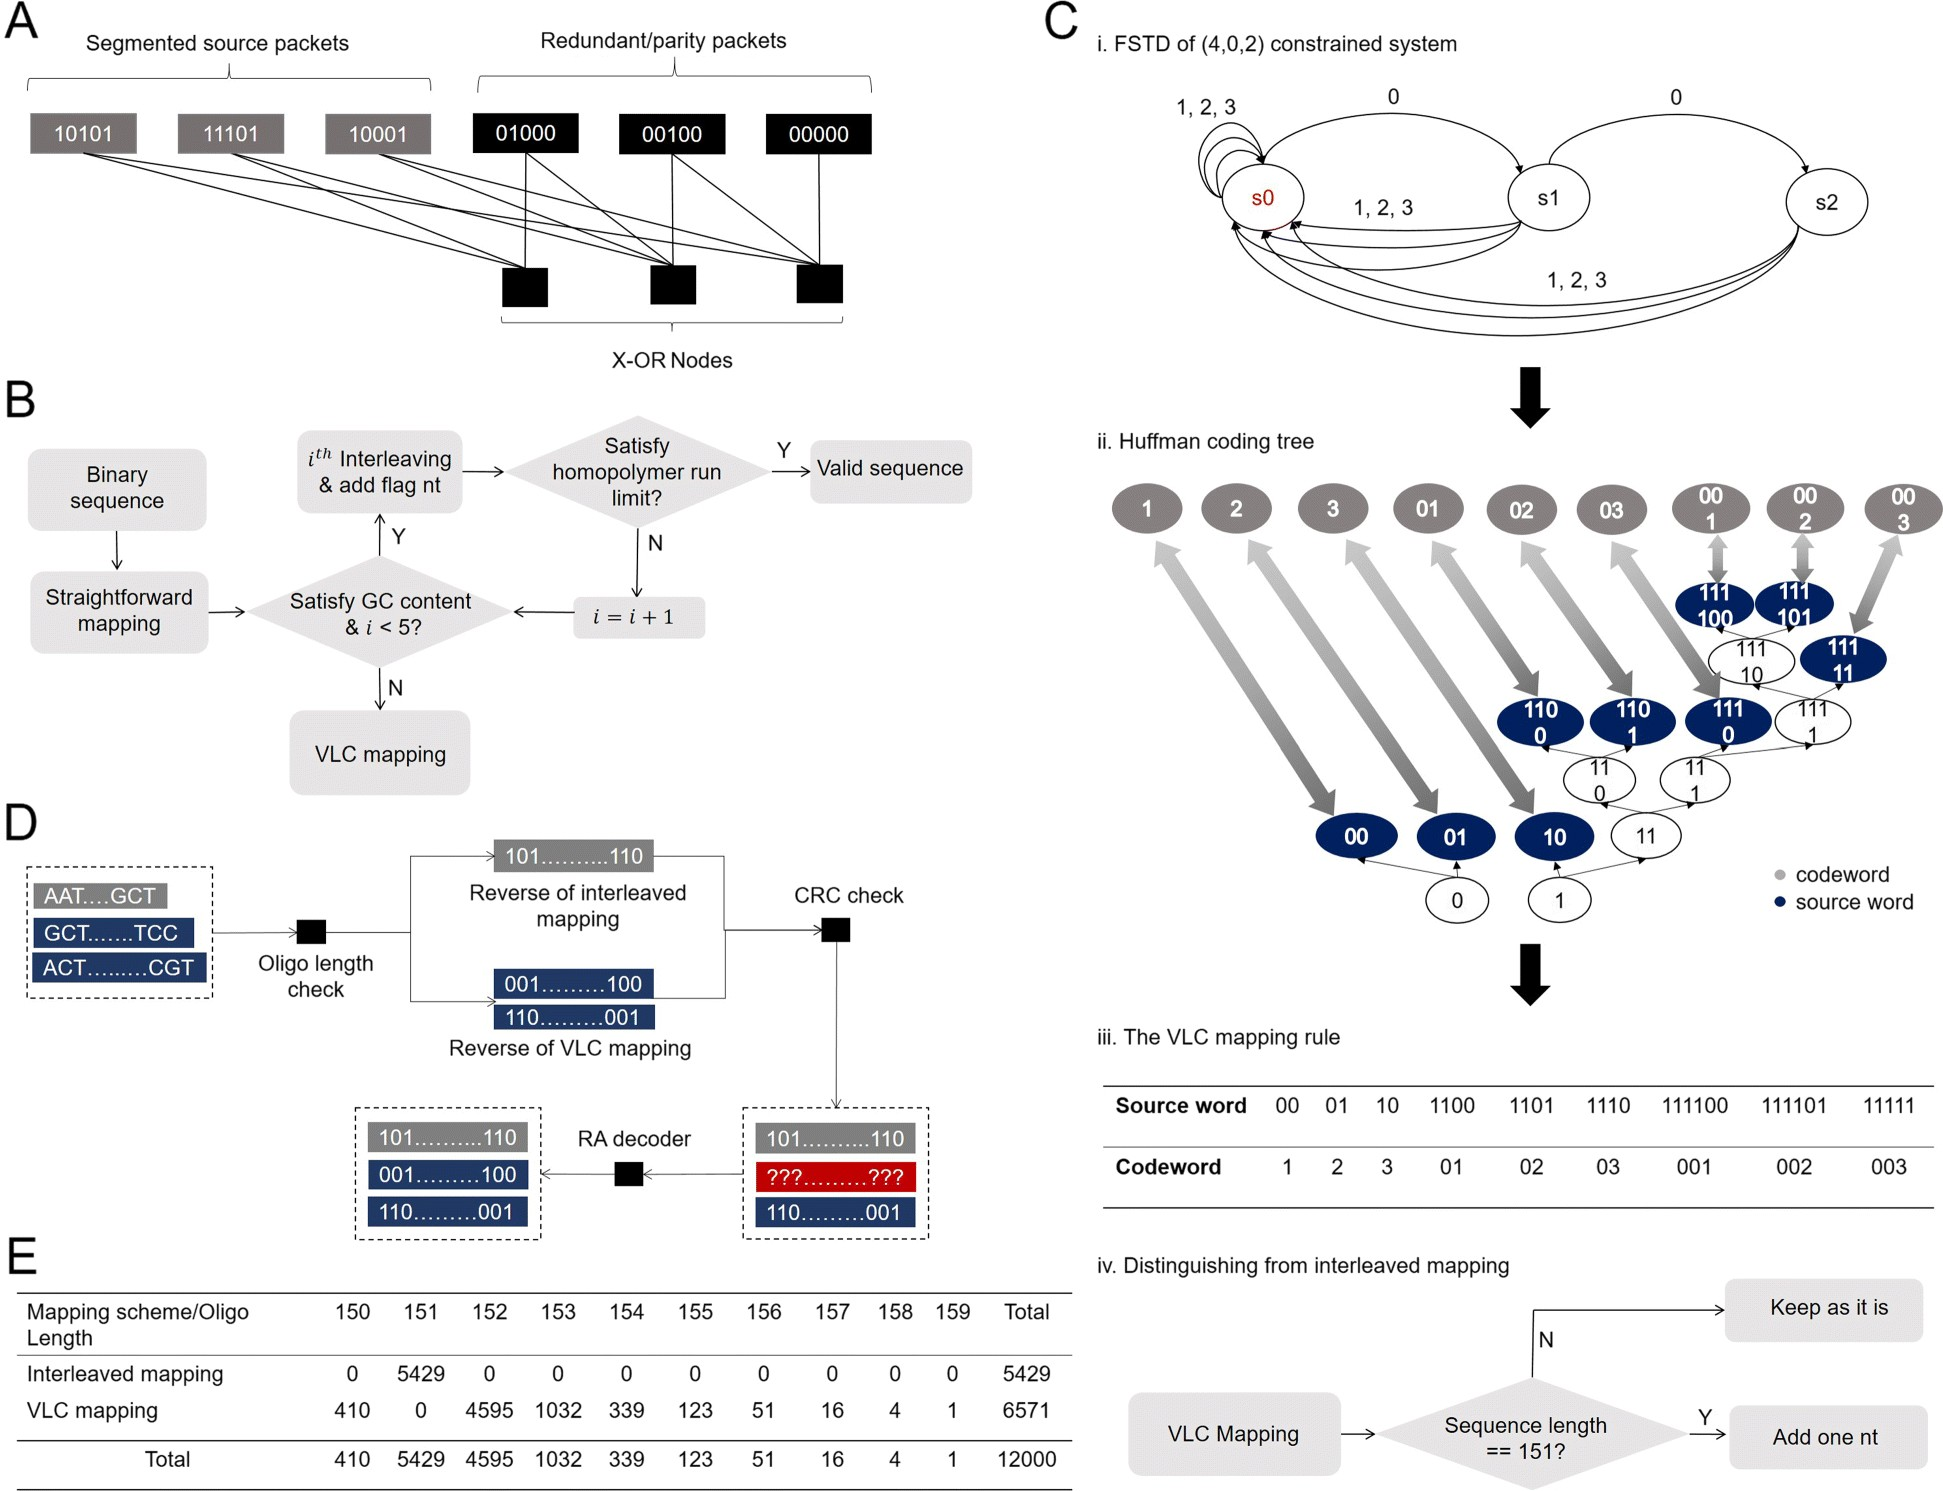
\includegraphics[width=\linewidth]{figure hybrid mapping.jpg}
\caption{The aforementioned illustration makes an attempt to better explain (RA) coding strategies and hybrid mapping by using the citation \cite{wang2019high} to show all the steps involved.\\
$(A)$ A rate 12 packet level RA code illustration using three source packets. The source packets connected to the ith X-OR node and the (i1)th parity packet are bit-wise mod-summed to create the ith parity packet at position.\\
The flowchart for the hybrid mapping is in $(B)$. By using binary-to-quaternary mapping, each binary sequence is initially mapped. In accordance with one of the interleaving patterns, the interleaved sequence with the flag nucleotide added at the end may pass the screening test, which examines the homopolymer and GC content, and thereby be output as a valid sequence. Otherwise, the original binary sequence will be sent to the variable-length constrained (VLC) mapping.
Otherwise, the variable-length constrained (VLC) mapping will be applied to the original binary sequence.
\\$(C.i)$ The $FSTD$ of a (4, 0, 2) constrained DNA storage system, where s0, s1 and s2 represent three different states that record the length of consecutive 0's (no transition) in the output (4, 0, 2) constrained sequences, and 0, 1, 2, and 3 represent four transition symbols that indicate the transitions among four nucleotide alphabets.\\
The creation of a "Huffman coding tree" $(C. ii)$. By aligning the source word with a high likelihood of occurrence with the codeword with a short length and vice versa, the Huffman coding tree increases the code rate. \\The VLC mapping rule $(C. iii)$. A look-up table between variable-length source words and variable-length transition codewords is produced by the alignment of the Huffman coding tree. \\$(C. iv)$ The method for allowing the decoder to distinguish between two mappings based on the length of the DNA sequence it receives.
\\The decoder's flowchart is in option $(D)$. Prior to performing the associative reverse, the decoder first determines the mapping strategy that the received sequence has employed. Next, the CRC check determines whether or not the reversed binary sequence contains errors. The RA decoder then attempts to recover every sequence that contains an error.
\\$(E)$ The distribution of DNA sequence lengths. The length of the resulting DNA sequences ranges from 150 nucleotides to 159 nucleotides, with the interleaved mapping only producing sequences longer than 151 nucleotides while the VLC mapping produces all other lengths.}
\label{fig10}
\end{figure*}

\section{Decoding}
As we mentioned in the previous sections, DNA decoding is the reverse process of encoding while retrieving data through the sequenced data. The sequencing of the DNA molecules is done in 2 main steps:
\begin{itemize}
    \item Sample collation and preparation involves gathering the A G T C from the organism of interest.
    \item Amplification, amplifying the DNA sequence means producing different copies of a selected gene segment.
\end{itemize}
After, they need to be decoded, which means that the string of sequenced DNA bases will be transformed back into 1's and 0's (digital data) \cite{alliance2021preserving}.

Most of the techniques used for encoding are possible to use in decoding ass well which we talked about some of them with methods of error correction to have minimum loss and maximum correctness. There are some points to be considered while doing the process of decoding:
\begin{itemize}
    \item Chemical and biological constraints which are in the synthesis and sequencing stages. There are several tools for sequencing like. NovogeneAIT, and Illumina, Focused power on the MiSeq System.
    \item Trying to check the quality of information and distribution of errors in set of sequences that are retrieved.
    \item Error correction methods which were introduced in the previous sections, like Reed-Solomon.
    \item Finally, the output should be checked so that the amount of loss, precision, and accuracy will be revealed.
\end{itemize}

\section{ECONOMICS OF DNA DATA STORAGE}
Talking about some economics, writing and reading DNA for storage are not practical to scale due to the chemical constrain in synthesising the data, but the trend shows that probably in some years it will change, and the synthesis cost will significantly drop Figure \ref{fig11}.

The synthesis cost is based on the factor in how the bits are encoded into the bases of DNA, and also the methods of DNA synthesis. Since today only a few companies are involved in this business and nowadays there is not any commercial application so it's difficult to understand the real future trend \cite{alliance2021preserving}.

However, Intelligence Advanced Research Projects Activity (IARPA) has set forth a projected roadmap toward a synthesis cost of \$1/gigabyte by 2024 and \$1/terabyte by 2030. IARPA is financing research in this field through their Molecular Information The storage (MIST) initiative.
Another significant illustration is that, according to the National Human Genome Research Institute (NHGRI), the cost of sequencing a human genome will drop from \$100 million in 2001 to \$1,000 in 2021. 
By the way, the human genome was fully sequenced in 2022 and its cost is less than \$1000.

Furthermore, the real benefit of DNA storage is given in the long-term storage compared with other traditional storage systems such as Tape or Cloud Archival \cite{rosenthal2012economics}.

\begin{figure}[ht]
\centering
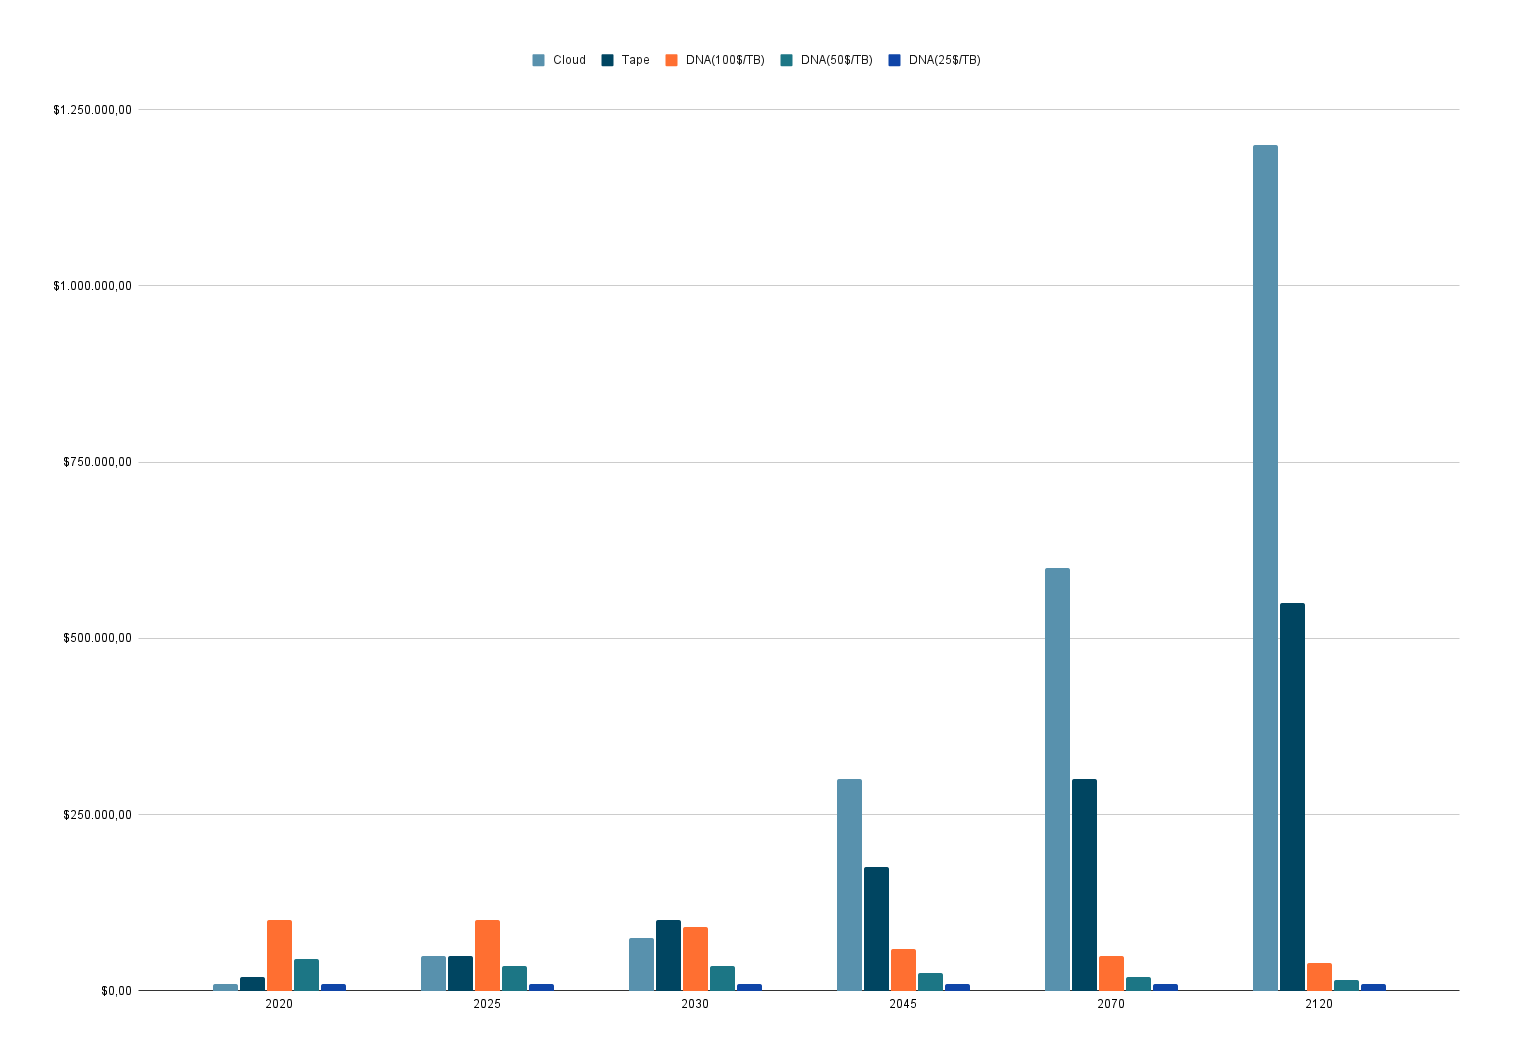
\includegraphics[width=\linewidth]{Figures/economicschart.png}
\caption{This is a chart that is showing the trend of the cost of the classic storage system versus the one that takes in
account of the cost of DNA during the time.
We can see the cloud is going to increase exponentially during this time this is due to the fact of the main idea of how
it works, the user needs to have access to their data at any time in a short amount of data. So the real competitor of
DNA storage is the Tape, for the explanation done in Kyders Law in the first section of the paper Tape and HDD are
following a log-like shape and the tech at some point will reach a bound. On the other side DNA storage is going
to decrease are predicted to decrease its cost this is due to the fact that, it is a sector in continuous expansion and
where research could take more consistent steps in the future to consolidate the techniques of encoding sequencing
and decoding of information \cite{alliance2021preserving}.}
\label{fig11}
\end{figure}

\section{Conclusion and future works}
\label{Conclusion}
Considering the stock of the current situation, the DNA data storage is a process that takes into account many small steps and every step is a brick to build this complex process. Each of these steps requires a thorough study of various subjects and therefore the involvement of various experts in the field. Focusing on this point, it is important to understand the difficulty in scaling this type of project, as today there is no figure able to cover all the various sectors and sciences to carry out the process. This reduces the speed and limits the process of developing this technology, as various figures must carry out each step.
\\
Taking a more specific example it can be said that two types of specialists collaborate, the engineers / mathematicians and the biologists / chemists for most of the research done in this field. However, they do not collaborate conjointly. In conclusion, no real solution has been found to the problems mentioned above, as a consequence not many investors are attracted since they do not see an immediate economic implication.
\\
In addition, today it is not possible to use querying operation on the DNA molecule, consequently, this compromises various problems in terms of timing. So, some recent papers are trying to implement this important operation, for example analysing the contrast between an object similar to the one you want to search for, while the other one is through deep learning techniques to reach a fast query matching.
\\
Regarding the future, since many papers are focusing on trying to solve the limits of writing speed on the molecule large-scale scalability of the storage system is not allowed given a long time. Another thing to consider just as important as the others are that DNA data storage could represent a valid alternative to reduce the pollution generated by the classic means of storage, representing a step towards a greener and cleaner future.


\bibliography{ourbib.bib}

\end{document} 